% Source: figures/figure_architecture.pdf, \label{fig:architecture} in sections/appendix.tex.
\begin{figure*}[h]
  \centering
  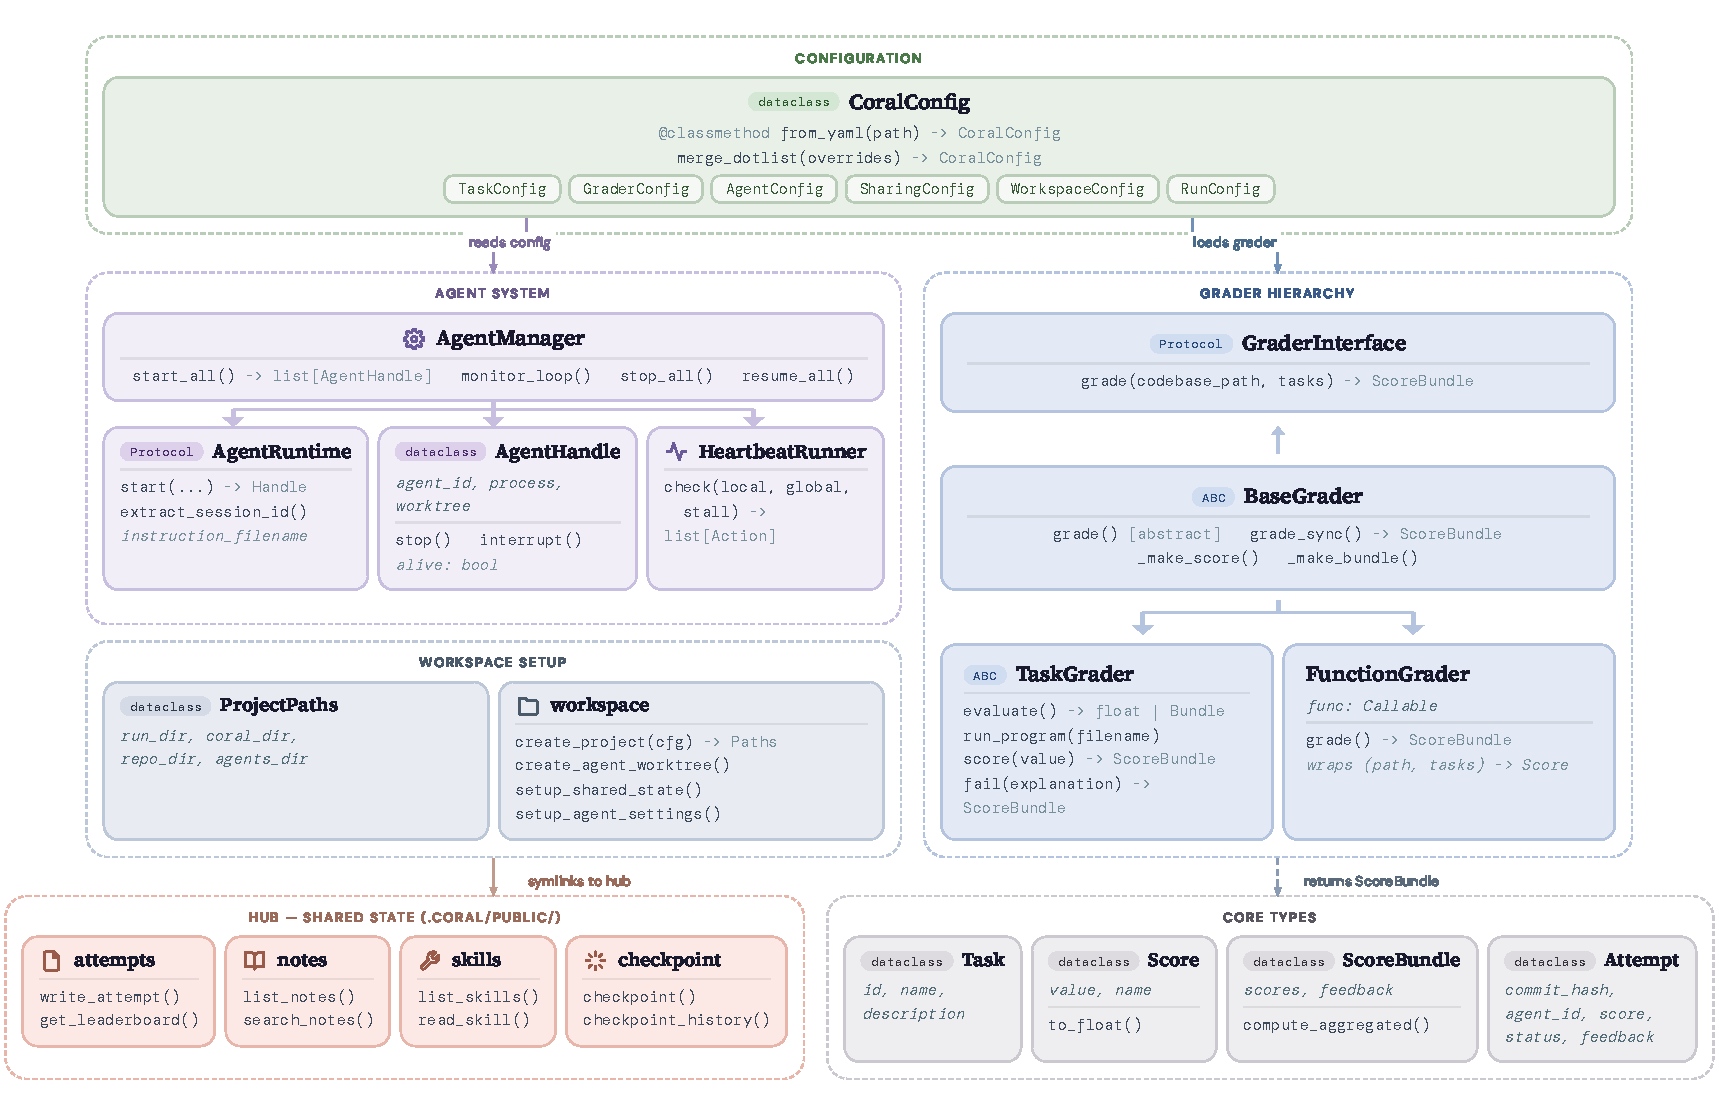
\includegraphics[width=\linewidth]{figures/srcs/11_architecture.pdf}
  \caption{Architecture of \method{}. The system is organized into six modules: \emph{Configuration} parses YAML task definitions; the \emph{Agent System} manages agent lifecycles and heartbeat-driven interventions; the \emph{Grader Hierarchy} provides a pluggable evaluation interface; \emph{Workspace Setup} creates isolated per-agent worktrees with symlinks to shared state; the \emph{Hub} stores shared persistent memory (attempts, notes, skills); and \emph{Core Types} define the data model. Arrows indicate primary data flow: configuration is consumed by both the agent system and grader loader; workspace setup creates symlinks into the hub; and graders return \texttt{ScoreBundle} objects defined in core types.}
  \label{fig:architecture}
\end{figure*}
